\documentclass[ASNA]{USG}
\usepackage{amsmath}
\usepackage{booktabs}
\usepackage{threeparttable}
\usepackage{array}
\usepackage{graphicx}
\usepackage{xurl}
\graphicspath{{images/}{./images/}}
\providecommand{\pkg}[1]{\textsf{#1}}
\providecommand{\proglang}[1]{\textsf{#1}}
\providecommand{\code}[1]{\texttt{#1}}
\providecommand{\tableref}[1]{Table~\ref{#1}}
\renewcommand{\thesection}{S\arabic{section}}
\renewcommand{\thetable}{S\arabic{table}}
\renewcommand{\thefigure}{S\arabic{figure}}
\makeatletter
\def\@@articletype{\rule[-4\@p@t]{4\@p@t}{15\@p@t}\hskip -0\@p@t%
  {\arttypefont\bf\uppercase{\letterspace to 1.15\naturalwidth{\@articletype}}}}
\makeatother
\usepackage{etoolbox}
\makeatletter
\patchcmd{\@maketitle}{
\includegraphics[width=56mm]{allergy.eps}}{}{}{}
\makeatother
\articletype{Supporting Information}
\received{}\revised{}\accepted{}
\journal{Journal of Forecasting}
\copyyear{2026}\volume{00}\startpage{1}\articledoi{10.1002/for.0000}
\begin{document}
\title{Supporting Information for ``Foundation or Formula? A Simulation-Based Comparison of
Google's TimesFM-3 and Classical Time-Series Models''}
\author[1]{Ebrahim Khaled Ebrahim}
\author[2]{Somaia Mohamed Ali}
\author[3]{Ahmed El-Kotory}
\authormark{EBRAHIM \textsc{et al.}}
\titlemark{Supporting Information}
\address[1]{\orgname{Alexandria University}, \orgaddress{\country{Egypt}}}
\address[2]{\orgname{Alexandria University}, \orgaddress{\country{Egypt}}}
\address[3]{\orgname{Alexandria University}, \orgaddress{\country{Egypt}}}
\corres{Ebrahim Khaled Ebrahim. \email{ebrahimkhaled@alexu.edu.eg}}
\abstract[Summary]{This file contains supporting information referred to in the main text as
Sections S1 to S7.}
\maketitle
\clearpage

\section{Results under the mean absolute percentage error}
\label{si:mape}

\tableref{tab:mape} reports mean MAPE by process, alongside the percentage of series on which
it cannot be computed. The D8 row illustrates the problem: every intermittent series contains a zero,
so MAPE is undefined for all of them, and the process on which TimesFM-3 achieves its largest
and most consistent advantage simply drops out of the comparison.

The rankings also move. On D4, MAPE places seasonal naive first (2.360) and TimesFM-3 second
(2.801), whereas MASE places AutoARIMA first at every length from $n = 48$. MAPE's asymmetry
between over- and under-forecasts is enough to reorder the methods on the same forecasts.

% generated by code/09_make_tables.py -- do not edit by hand
\begin{table}[!htbp]
\centering
\begin{threeparttable}
\caption{Mean MAPE over $h = 1,\dots,12$ and percentage of series on which MAPE is undefined.}
\label{tab:mape}
\small
\begin{tabular}{lrrrrrrr}
\toprule
DGP & \% undefined & Seas.\ naive & Theta & AutoETS & AutoARIMA & Combin. & \textbf{TimesFM-3} \\
\midrule
D1 & 0\% & 2.785 & 2.737 & 2.681 & 2.336 & 2.501 & \textbf{2.283} \\
D2 & 0\% & 3.291 & 3.341 & 3.277 & 2.696 & 2.971 & \textbf{2.641} \\
D3 & 0\% & 9.509 & 9.278 & 9.875 & 10.078 & 9.393 & \textbf{9.214} \\
D4 & 0\% & \textbf{2.360} & 7.471 & 4.986 & 2.862 & 4.538 & 2.801 \\
D5 & 0\% & 2.971 & 3.583 & 3.270 & 2.436 & 2.916 & \textbf{2.256} \\
D6 & 0\% & 2.011 & 2.379 & 1.835 & 1.902 & 1.925 & \textbf{1.822} \\
D7 & 0\% & 7.634 & 4.631 & 2.979 & 2.538 & 2.767 & \textbf{2.184} \\
D8 & 100\% & --- & --- & --- & --- & --- & --- \\
D9 & 0\% & 1.861 & 1.769 & 1.741 & 1.470 & 1.599 & \textbf{1.457} \\
\bottomrule
\end{tabular}
\begin{tablenotes}[flushleft]\footnotesize
\item \textit{Note:} On the intermittent process D8 every series contains a zero, so MAPE cannot be computed for it. The best value in each row is in bold.
\end{tablenotes}
\end{threeparttable}
\end{table}


\section{Monte Carlo standard errors}
\label{si:mcse}

\tableref{tab:si-mcse} gives the mean MASE of the six methods of the main design in every cell,
with its Monte Carlo standard error.

\begin{table}[!htbp]
\centering
\begin{threeparttable}
\caption{Mean MASE and Monte Carlo standard errors, main design.}
\label{tab:si-mcse}
\scriptsize\setlength{\tabcolsep}{3pt}\renewcommand{\arraystretch}{0.9}
\begin{tabular}{llcccccc}
\toprule
DGP & $n$ & Seasonal naive & Theta & AutoETS & AutoARIMA & Combination & TimesFM-3 \\
\midrule
D1 & 24 & 1.646 (0.056) & 1.682 (0.055) & 1.568 (0.050) & 1.485 (0.048) & 1.538 (0.048) & 1.417 (0.042) \\
D1 & 48 & 1.625 (0.058) & 1.586 (0.055) & 1.570 (0.054) & 1.415 (0.043) & 1.478 (0.048) & 1.381 (0.039) \\
D1 & 96 & 1.626 (0.054) & 1.572 (0.053) & 1.564 (0.053) & 1.324 (0.039) & 1.435 (0.044) & 1.307 (0.033) \\
D1 & 200 & 1.615 (0.061) & 1.576 (0.057) & 1.576 (0.057) & 1.266 (0.035) & 1.417 (0.046) & 1.254 (0.033) \\
D2 & 24 & 1.905 (0.066) & 2.003 (0.073) & 1.886 (0.069) & 1.708 (0.087) & 1.788 (0.065) & 1.675 (0.062) \\
D2 & 48 & 1.838 (0.068) & 1.860 (0.069) & 1.834 (0.068) & 1.575 (0.053) & 1.688 (0.058) & 1.518 (0.042) \\
D2 & 96 & 1.810 (0.057) & 1.812 (0.057) & 1.811 (0.057) & 1.517 (0.038) & 1.643 (0.045) & 1.455 (0.035) \\
D2 & 200 & 1.922 (0.067) & 1.919 (0.067) & 1.921 (0.067) & 1.374 (0.034) & 1.654 (0.050) & 1.383 (0.033) \\
D3 & 24 & 4.411 (0.213) & 4.483 (0.219) & 4.892 (0.235) & 5.275 (0.256) & 4.659 (0.224) & 4.656 (0.236) \\
D3 & 48 & 4.252 (0.208) & 4.179 (0.206) & 4.547 (0.207) & 4.679 (0.239) & 4.313 (0.203) & 4.274 (0.205) \\
D3 & 96 & 4.125 (0.191) & 4.135 (0.189) & 3.938 (0.179) & 3.940 (0.179) & 3.871 (0.172) & 4.023 (0.177) \\
D3 & 200 & 4.512 (0.210) & 4.427 (0.211) & 4.275 (0.199) & 4.195 (0.201) & 4.199 (0.199) & 4.297 (0.198) \\
D4 & 24 & 1.029 (0.026) & 4.146 (0.110) & 3.602 (0.101) & 2.284 (0.079) & 3.084 (0.072) & 1.321 (0.031) \\
D4 & 48 & 1.021 (0.024) & 1.944 (0.048) & 1.720 (0.032) & 1.014 (0.030) & 1.395 (0.028) & 1.295 (0.027) \\
D4 & 96 & 1.005 (0.024) & 2.910 (0.078) & 2.407 (0.055) & 0.886 (0.020) & 1.839 (0.040) & 1.124 (0.022) \\
D4 & 200 & 1.053 (0.022) & 4.155 (0.117) & 1.085 (0.024) & 0.886 (0.021) & 1.700 (0.043) & 1.161 (0.020) \\
D5 & 24 & 1.139 (0.038) & 3.154 (0.102) & 3.025 (0.093) & 1.574 (0.043) & 2.474 (0.069) & 1.152 (0.038) \\
D5 & 48 & 1.108 (0.032) & 0.956 (0.038) & 0.741 (0.027) & 0.717 (0.024) & 0.731 (0.023) & 0.815 (0.029) \\
D5 & 96 & 1.076 (0.033) & 0.757 (0.025) & 0.761 (0.029) & 0.732 (0.027) & 0.713 (0.027) & 0.761 (0.029) \\
D5 & 200 & 1.040 (0.030) & 0.759 (0.020) & 0.681 (0.024) & 0.626 (0.022) & 0.645 (0.022) & 0.689 (0.024) \\
D6 & 24 & 0.801 (0.025) & 1.327 (0.038) & 0.766 (0.024) & 0.802 (0.025) & 0.837 (0.025) & 0.807 (0.036) \\
D6 & 48 & 0.947 (0.028) & 1.115 (0.031) & 0.869 (0.023) & 0.925 (0.027) & 0.924 (0.025) & 0.825 (0.022) \\
D6 & 96 & 1.006 (0.028) & 0.963 (0.026) & 0.905 (0.023) & 0.920 (0.023) & 0.916 (0.023) & 0.865 (0.021) \\
D6 & 200 & 0.934 (0.023) & 0.840 (0.017) & 0.825 (0.017) & 0.833 (0.017) & 0.827 (0.017) & 0.844 (0.019) \\
D7 & 24 & 5.417 (0.080) & 3.179 (0.058) & 1.272 (0.042) & 1.083 (0.037) & 1.680 (0.048) & 1.142 (0.033) \\
D7 & 48 & 4.243 (0.067) & 2.262 (0.048) & 1.602 (0.061) & 1.076 (0.051) & 0.970 (0.038) & 0.751 (0.022) \\
D7 & 96 & 1.655 (0.042) & 0.821 (0.020) & 1.305 (0.047) & 1.329 (0.048) & 1.097 (0.036) & 0.959 (0.032) \\
D7 & 200 & 0.917 (0.026) & 1.301 (0.031) & 0.966 (0.028) & 0.994 (0.030) & 0.954 (0.027) & 0.933 (0.025) \\
D8 & 24 & 1.019 (0.054) & 0.999 (0.034) & 1.047 (0.058) & 0.996 (0.032) & 1.010 (0.039) & 0.780 (0.031) \\
D8 & 48 & 1.066 (0.066) & 0.984 (0.036) & 0.988 (0.033) & 0.962 (0.024) & 0.974 (0.028) & 0.708 (0.030) \\
D8 & 96 & 0.932 (0.047) & 0.923 (0.017) & 0.926 (0.015) & 0.924 (0.015) & 0.923 (0.015) & 0.683 (0.022) \\
D8 & 200 & 1.005 (0.052) & 0.943 (0.017) & 0.939 (0.015) & 0.939 (0.015) & 0.940 (0.015) & 0.694 (0.023) \\
D9 & 24 & 1.547 (0.061) & 1.518 (0.057) & 1.454 (0.057) & 1.372 (0.057) & 1.404 (0.054) & 1.321 (0.049) \\
D9 & 48 & 1.588 (0.056) & 1.486 (0.054) & 1.476 (0.053) & 1.244 (0.041) & 1.353 (0.046) & 1.239 (0.039) \\
D9 & 96 & 1.430 (0.051) & 1.342 (0.048) & 1.333 (0.048) & 1.098 (0.034) & 1.213 (0.040) & 1.104 (0.034) \\
D9 & 200 & 1.577 (0.056) & 1.503 (0.053) & 1.504 (0.053) & 1.190 (0.032) & 1.341 (0.042) & 1.200 (0.035) \\
\bottomrule
\end{tabular}
\begin{tablenotes}[flushleft]\footnotesize
\item \textit{Note:} Mean MASE over $h = 1, \dots, 12$ with its Monte Carlo standard error in parentheses (standard deviation over the 200 replications divided by $\sqrt{200}$).
\end{tablenotes}
\end{threeparttable}
\end{table}


\section{Coverage by process}
\label{si:coverage}

\tableref{tab:si-coverage} gives the empirical coverage of the nominal 80\% intervals of the four
foundation-model configurations and of AutoARIMA and AutoETS, by process.

\begin{table}[!htbp]
\centering
\begin{threeparttable}
\caption{Coverage of 80\% prediction intervals by process.}
\label{tab:si-coverage}
\small\setlength{\tabcolsep}{4pt}
\begin{tabular}{lcccccc}
\toprule
Process & TimesFM-3 & TimesFM-3 (eval.) & TimesFM-2.5 & Chronos-Bolt & AutoARIMA & AutoETS \\
\midrule
D1 & 0.817 & 0.819 & 0.787 & 0.814 & 0.777 & 0.852 \\
D2 & 0.817 & 0.818 & 0.782 & 0.824 & 0.766 & 0.874 \\
D3 & 0.704 & 0.707 & 0.703 & 0.721 & 0.706 & 0.618 \\
D4 & 0.846 & 0.856 & 0.810 & 0.769 & 0.756 & 0.661 \\
D5 & 0.818 & 0.830 & 0.799 & 0.833 & 0.724 & 0.686 \\
D6 & 0.859 & 0.873 & 0.913 & 0.921 & 0.986 & 0.987 \\
D7 & 0.845 & 0.848 & 0.894 & 0.968 & 0.833 & 0.765 \\
D8 & 0.818 & 0.869 & 0.835 & 0.846 & 0.836 & 0.843 \\
D9 & 0.807 & 0.809 & 0.783 & 0.810 & 0.760 & 0.825 \\
\bottomrule
\end{tabular}
\begin{tablenotes}[flushleft]\footnotesize
\item \textit{Note:} Empirical coverage of the nominal 80\% interval $[q_{0.1}, q_{0.9}]$, averaged over lengths and replications; series-cluster bootstrap Monte Carlo SE at most 0.016.
\end{tablenotes}
\end{threeparttable}
\end{table}


\section{Response-surface regressions}
\label{si:response}

Tables~\ref{tab:si-response} and~\ref{tab:si-response2} report the regressions summarised in the section of the main text on
randomised parameters and departures from the assumptions.

\begin{table}[!htbp]
\centering
\begin{threeparttable}
\caption{Response-surface regressions of the robustness study, processes D1--D4.}
\label{tab:si-response}
\scriptsize
\begin{tabular}{llcccc}
\toprule
Process & Term & Coefficient & 95\% interval & $p$ & $R^2$ \\
\midrule
D1 & version: est period & 0.000 & [-0.002, 0.002] & 0.945 & 0.003 \\
D1 & version: heavy tail & -0.022 & [-0.048, 0.004] & 0.091 & 0.003 \\
D1 & version: outliers & -0.010 & [-0.031, 0.010] & 0.335 & 0.003 \\
D1 & $\log_2 n$ & 0.004 & [-0.010, 0.019] & 0.552 & 0.003 \\
D1 & parameter phi & -0.013 & [-0.031, 0.005] & 0.161 & 0.003 \\
D1 & parameter sigma & 0.006 & [-0.010, 0.021] & 0.476 & 0.003 \\
D2 & version: est period & -0.000 & [-0.001, 0.001] & 0.795 & 0.012 \\
D2 & version: heavy tail & -0.016 & [-0.041, 0.009] & 0.207 & 0.012 \\
D2 & version: outliers & 0.004 & [-0.014, 0.021] & 0.661 & 0.012 \\
D2 & $\log_2 n$ & -0.002 & [-0.017, 0.013] & 0.828 & 0.012 \\
D2 & parameter phi & -0.031 & [-0.050, -0.012] & 0.002 & 0.012 \\
D2 & parameter sigma & 0.010 & [-0.007, 0.027] & 0.232 & 0.012 \\
D2 & parameter theta & 0.005 & [-0.012, 0.022] & 0.567 & 0.012 \\
D3 & version: est period & 0.000 & [-0.004, 0.005] & 0.876 & 0.006 \\
D3 & version: heavy tail & 0.020 & [-0.036, 0.075] & 0.487 & 0.006 \\
D3 & version: outliers & -0.004 & [-0.039, 0.032] & 0.843 & 0.006 \\
D3 & $\log_2 n$ & 0.014 & [-0.021, 0.049] & 0.422 & 0.006 \\
D3 & parameter phi & -0.046 & [-0.088, -0.004] & 0.030 & 0.006 \\
D3 & parameter sigma & -0.004 & [-0.043, 0.035] & 0.844 & 0.006 \\
D3 & parameter theta & 0.017 & [-0.022, 0.056] & 0.396 & 0.006 \\
D3 & parameter drift & -0.010 & [-0.049, 0.029] & 0.608 & 0.006 \\
D4 & version: est period & -0.004 & [-0.009, 0.001] & 0.141 & 0.255 \\
D4 & version: heavy tail & 0.061 & [0.028, 0.095] & 0.000 & 0.255 \\
D4 & version: outliers & -0.219 & [-0.260, -0.178] & 0.000 & 0.255 \\
D4 & $\log_2 n$ & 0.258 & [0.229, 0.287] & 0.000 & 0.255 \\
D4 & parameter phi & -0.055 & [-0.089, -0.021] & 0.002 & 0.255 \\
D4 & parameter sigma & 0.047 & [0.012, 0.082] & 0.009 & 0.255 \\
D4 & parameter Phi & 0.110 & [0.075, 0.145] & 0.000 & 0.255 \\
D4 & parameter amp & -0.038 & [-0.071, -0.006] & 0.020 & 0.255 \\
\bottomrule
\end{tabular}
\begin{tablenotes}[flushleft]\footnotesize
\item \textit{Note:} One ordinary least-squares regression per process of the per-series $\log_2$ ratio of the MASE of TimesFM-3 to that of AutoARIMA on $\log_2 n$ (not standardised), the version (reference: random parameters with Gaussian innovations) and the drawn parameters, each standardised to mean 0 and standard deviation 1. Standard errors are clustered by parameter draw, because the four versions of a draw share its parameters and normal draws; 3\,200 series per process (3\,188 for D8, where series with a zero MASE denominator are excluded). Positive coefficients move the ratio against TimesFM-3.
\end{tablenotes}
\end{threeparttable}
\end{table}

\begin{table}[!htbp]
\centering
\begin{threeparttable}
\caption{Response-surface regressions of the robustness study, processes D5--D9.}
\label{tab:si-response2}
\scriptsize
\begin{tabular}{llcccc}
\toprule
Process & Term & Coefficient & 95\% interval & $p$ & $R^2$ \\
\midrule
D5 & version: est period & -0.086 & [-0.111, -0.061] & 0.000 & 0.090 \\
D5 & version: heavy tail & -0.002 & [-0.039, 0.036] & 0.934 & 0.090 \\
D5 & version: outliers & -0.151 & [-0.191, -0.111] & 0.000 & 0.090 \\
D5 & $\log_2 n$ & 0.147 & [0.119, 0.174] & 0.000 & 0.090 \\
D5 & parameter sigma & 0.032 & [-0.001, 0.065] & 0.056 & 0.090 \\
D5 & parameter amp & -0.021 & [-0.054, 0.012] & 0.214 & 0.090 \\
D5 & parameter alpha & -0.017 & [-0.050, 0.016] & 0.303 & 0.090 \\
D5 & parameter beta & -0.008 & [-0.042, 0.026] & 0.659 & 0.090 \\
D5 & parameter gamma & 0.031 & [-0.003, 0.064] & 0.075 & 0.090 \\
D5 & parameter trend & 0.010 & [-0.022, 0.042] & 0.522 & 0.090 \\
D6 & version: est period & -0.002 & [-0.004, 0.000] & 0.066 & 0.022 \\
D6 & version: heavy tail & 0.018 & [-0.022, 0.058] & 0.384 & 0.022 \\
D6 & version: outliers & -0.023 & [-0.053, 0.008] & 0.140 & 0.022 \\
D6 & $\log_2 n$ & -0.046 & [-0.080, -0.012] & 0.007 & 0.022 \\
D6 & parameter sigma & -0.029 & [-0.070, 0.011] & 0.154 & 0.022 \\
D6 & parameter jump sd & -0.038 & [-0.071, -0.004] & 0.028 & 0.022 \\
D6 & parameter break pos & -0.047 & [-0.085, -0.009] & 0.016 & 0.022 \\
D6 & parameter sigma level & 0.029 & [-0.006, 0.064] & 0.100 & 0.022 \\
D6 & parameter jump sign & -0.011 & [-0.047, 0.025] & 0.549 & 0.022 \\
D7 & version: est period & -0.002 & [-0.011, 0.008] & 0.741 & 0.022 \\
D7 & version: heavy tail & -0.031 & [-0.081, 0.018] & 0.216 & 0.022 \\
D7 & version: outliers & -0.045 & [-0.094, 0.005] & 0.075 & 0.022 \\
D7 & $\log_2 n$ & 0.034 & [-0.007, 0.075] & 0.103 & 0.022 \\
D7 & parameter sigma & -0.048 & [-0.100, 0.004] & 0.070 & 0.022 \\
D7 & parameter r & 0.068 & [0.017, 0.120] & 0.009 & 0.022 \\
D7 & parameter infl pos & -0.081 & [-0.136, -0.027] & 0.003 & 0.022 \\
D7 & parameter K & 0.011 & [-0.039, 0.061] & 0.678 & 0.022 \\
D8 & version: est period & -0.001 & [-0.003, 0.001] & 0.355 & 0.203 \\
D8 & version: heavy tail & -0.047 & [-0.078, -0.016] & 0.003 & 0.203 \\
D8 & version: outliers & -0.025 & [-0.043, -0.007] & 0.007 & 0.203 \\
D8 & $\log_2 n$ & -0.096 & [-0.162, -0.030] & 0.004 & 0.203 \\
D8 & parameter p & 0.509 & [0.422, 0.596] & 0.000 & 0.203 \\
D8 & parameter lam & 0.008 & [-0.064, 0.080] & 0.836 & 0.203 \\
D9 & version: est period & -0.002 & [-0.003, -0.000] & 0.045 & 0.000 \\
D9 & version: heavy tail & -0.007 & [-0.032, 0.018] & 0.592 & 0.000 \\
D9 & version: outliers & -0.013 & [-0.032, 0.007] & 0.196 & 0.000 \\
D9 & $\log_2 n$ & -0.003 & [-0.018, 0.012] & 0.719 & 0.000 \\
D9 & parameter phi & 0.002 & [-0.017, 0.021] & 0.814 & 0.000 \\
D9 & parameter a & -0.001 & [-0.019, 0.017] & 0.923 & 0.000 \\
D9 & parameter b & -0.001 & [-0.018, 0.016] & 0.927 & 0.000 \\
\bottomrule
\end{tabular}
\begin{tablenotes}[flushleft]\footnotesize
\item \textit{Note:} One ordinary least-squares regression per process of the per-series $\log_2$ ratio of the MASE of TimesFM-3 to that of AutoARIMA on $\log_2 n$ (not standardised), the version (reference: random parameters with Gaussian innovations) and the drawn parameters, each standardised to mean 0 and standard deviation 1. Standard errors are clustered by parameter draw, because the four versions of a draw share its parameters and normal draws; 3\,200 series per process (3\,188 for D8, where series with a zero MASE denominator are excluded). Positive coefficients move the ratio against TimesFM-3.
\end{tablenotes}
\end{threeparttable}
\end{table}


\section{Additional results moved from the main text}
\label{si:additional}

\tableref{tab:d8metrics} gives the error measures of the six pre-registered methods on the
intermittent process D8, and \tableref{tab:croston} compares TimesFM-3 with six Croston-family methods.
\tableref{tab:ranges} lists the parameter ranges of the randomised design, Figure~S1 shows accuracy by
forecast horizon, and Figure~S2 shows how the relative accuracy of TimesFM-3 and AutoARIMA varies with the
drawn parameters. \tableref{tab:mase} gives the mean MASE of every method in every cell of the main
design, summarised in Figure~2 of the main text.

% generated by code/09_make_tables.py -- do not edit by hand
\begin{table}[!htbp]
\centering
\begin{threeparttable}
\caption{Accuracy on the intermittent process D8 under four error measures.}
\label{tab:d8metrics}
\small\setlength{\tabcolsep}{4pt}
\begin{tabular}{llrrrrrr}
\toprule
Metric & $n$ & Seas.\ naive & Theta & AutoETS & AutoARIMA & Combin. & \textbf{TimesFM-3} \\
\midrule
MASE & 24 & 1.019 & 0.999 & 1.047 & 0.996 & 1.010 & \textbf{0.780} \\
 & 48 & 1.066 & 0.984 & 0.988 & 0.962 & 0.974 & \textbf{0.708} \\
 & 96 & 0.932 & 0.923 & 0.926 & 0.924 & 0.923 & \textbf{0.683} \\
 & 200 & 1.005 & 0.943 & 0.939 & 0.939 & 0.940 & \textbf{0.694} \\
\addlinespace
RMSSE & 24 & 0.940 & 0.791 & 0.792 & \textbf{0.765} & 0.775 & 0.806 \\
 & 48 & 0.937 & 0.746 & 0.726 & \textbf{0.718} & 0.724 & 0.774 \\
 & 96 & 0.875 & 0.707 & \textbf{0.697} & 0.698 & 0.697 & 0.775 \\
 & 200 & 0.923 & 0.718 & \textbf{0.706} & 0.706 & 0.706 & 0.797 \\
\addlinespace
sMAPE & 24 & \textbf{86.696} & 172.741 & 169.988 & 165.908 & 170.489 & 191.774 \\
 & 48 & \textbf{84.690} & 172.522 & 170.746 & 170.622 & 171.026 & 196.183 \\
 & 96 & \textbf{84.171} & 170.801 & 169.574 & 170.065 & 169.949 & 197.610 \\
 & 200 & \textbf{85.990} & 170.003 & 169.189 & 169.315 & 169.236 & 198.556 \\
\addlinespace
Pinball & 24 & 0.634 & 0.395 & 0.402 & 0.380 & 0.388 & \textbf{0.325} \\
 & 48 & 0.653 & 0.381 & 0.368 & 0.360 & 0.365 & \textbf{0.307} \\
 & 96 & 0.614 & 0.348 & 0.341 & 0.341 & 0.341 & \textbf{0.288} \\
 & 200 & 0.628 & 0.354 & 0.344 & 0.345 & 0.345 & \textbf{0.291} \\
\bottomrule
\end{tabular}
\begin{tablenotes}[flushleft]\footnotesize
\item \textit{Note:} Means over $h = 1,\dots,12$ and 200 replications per length. The pinball loss is averaged over the nine deciles. Lower is better; the best value in each row is in bold.
\end{tablenotes}
\end{threeparttable}
\end{table}


% generated by code/10_croston_d8.py -- do not edit by hand
\begin{table}[!htbp]
\centering
\begin{threeparttable}
\caption{Intermittent-demand baselines on the process D8 (post hoc analysis).}
\label{tab:croston}
\footnotesize\setlength{\tabcolsep}{3pt}
\begin{tabular}{llrrrrrrrr}
\toprule
Metric & $n$ & Croston & Croston-opt & Croston-SBA & ADIDA & IMAPA & TSB & AutoARIMA & \textbf{TimesFM-3} \\
\midrule
MASE & 24 & 1.042 & 1.024 & 1.025 & 0.972 & 0.972 & 0.971 & 0.996 & \textbf{0.780} \\
 & 48 & 0.990 & 0.992 & 0.974 & 0.947 & 0.954 & 0.966 & 0.962 & \textbf{0.708} \\
 & 96 & 0.935 & 0.948 & 0.921 & 0.926 & 0.923 & 0.916 & 0.924 & \textbf{0.683} \\
 & 200 & 0.947 & 0.948 & 0.934 & 0.941 & 0.942 & 0.948 & 0.939 & \textbf{0.694} \\
\addlinespace
RMSSE & 24 & 0.769 & 0.758 & 0.763 & \textbf{0.753} & 0.757 & 0.764 & 0.765 & 0.806 \\
 & 48 & 0.722 & 0.726 & 0.718 & \textbf{0.717} & 0.722 & 0.733 & 0.718 & 0.774 \\
 & 96 & 0.696 & 0.702 & \textbf{0.694} & 0.700 & 0.701 & 0.716 & 0.698 & 0.775 \\
 & 200 & 0.709 & 0.710 & 0.707 & 0.709 & 0.712 & 0.730 & \textbf{0.706} & 0.797 \\
\bottomrule
\end{tabular}
\begin{tablenotes}[flushleft]\footnotesize
\item \textit{Note:} Mean MASE and RMSSE over $h = 1,\dots,12$ and 200 replications per length. Croston-opt is Croston's method with optimised smoothing parameters and Croston-SBA the Syntetos--Boylan approximation. Lower is better; the best value in each row is in bold.
\end{tablenotes}
\end{threeparttable}
\end{table}


\begin{table}[!htbp]
\centering
\begin{threeparttable}
\caption{Parameter ranges of the randomised-parameter design.}
\label{tab:ranges}
\small\setlength{\tabcolsep}{4pt}
\begin{tabular}{ll}
\toprule
ID & Parameters, each drawn uniformly on the stated interval \\
\midrule
D1 & $\phi \in [0.10, 0.95]$, $\sigma \in [1, 5]$ \\
D2 & $\phi \in [0.10, 0.90]$, $\theta \in [-0.6, 0.8]$, $\sigma \in [1, 5]$ \\
D3 & $\phi \in [-0.5, 0.8]$, $\theta \in [-0.5, 0.6]$, drift $\in [0, 0.6]$, $\sigma \in [1, 5]$ \\
D4 & $\phi \in [0.1, 0.8]$, $\Phi \in [0.1, 0.8]$, seasonal amplitude $\in [5, 20]$, $\sigma \in [1, 5]$ \\
D5 & $\alpha \in [0.05, 0.5]$, $\beta \in [0.001, 0.03]$, $\gamma \in [0.05, 0.3]$, initial trend $\in [0, 0.5]$, amplitude $\in [5, 20]$, $\sigma \in [1, 5]$ \\
D6 & jump $\in [3, 15]\,\sigma$ with random sign, break at $[0.50, 0.85]\,n$, level noise $\in [0.2, 1]$, $\sigma \in [1, 5]$ \\
D7 & $r \in [0.04, 0.15]$, inflection at $[0.4, 0.8](n + H)$, $K \in [100, 250]$, $\sigma \in [1, 6]$ \\
D8 & demand probability $p \in [0.1, 0.6]$, size $1 + \mathrm{Pois}(\lambda)$ with $\lambda \in [1, 8]$ \\
D9 & $\phi \in [0.1, 0.9]$, $a \in [0.05, 0.15]$, $b \in [0.75, 0.90]$; if $a + b \geq 0.98$, $b$ is set to $0.97 - a$ \\
\bottomrule
\end{tabular}
\begin{tablenotes}[flushleft]\footnotesize
\item \textit{Note:} Parameters not listed are as in Table~2 of the main text. The intervals contain the
fixed values of the main design. The rule for D9 keeps the conditional variance stationary and puts
a small point mass at $b = 0.97 - a$. Seeds are disjoint from those of the main design; the four
versions share the parameter draws and, except for the heavy-tailed D8 sizes, the underlying normal
draws.
\end{tablenotes}
\end{threeparttable}
\end{table}

\begin{figure}[!htbp]
\centering
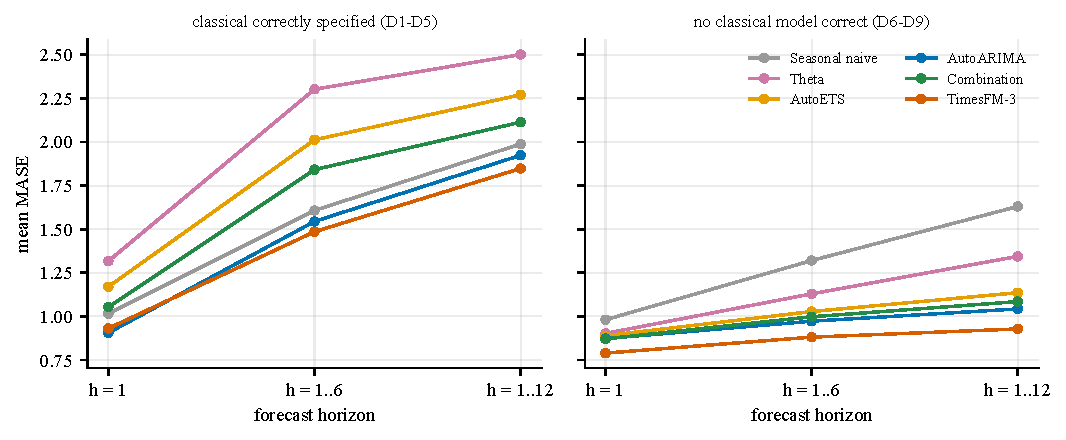
\includegraphics[width=\textwidth]{../figures/fig4_horizon.pdf}
\caption{Mean MASE by forecast horizon, averaged within each regime. Left: D1--D5, for which a classical
family is correctly specified. Right: D6--D9, for which none is, or only in the conditional mean (D9).}
\label{fig:si-horizon}
\end{figure}

\begin{figure}[!htbp]
\centering
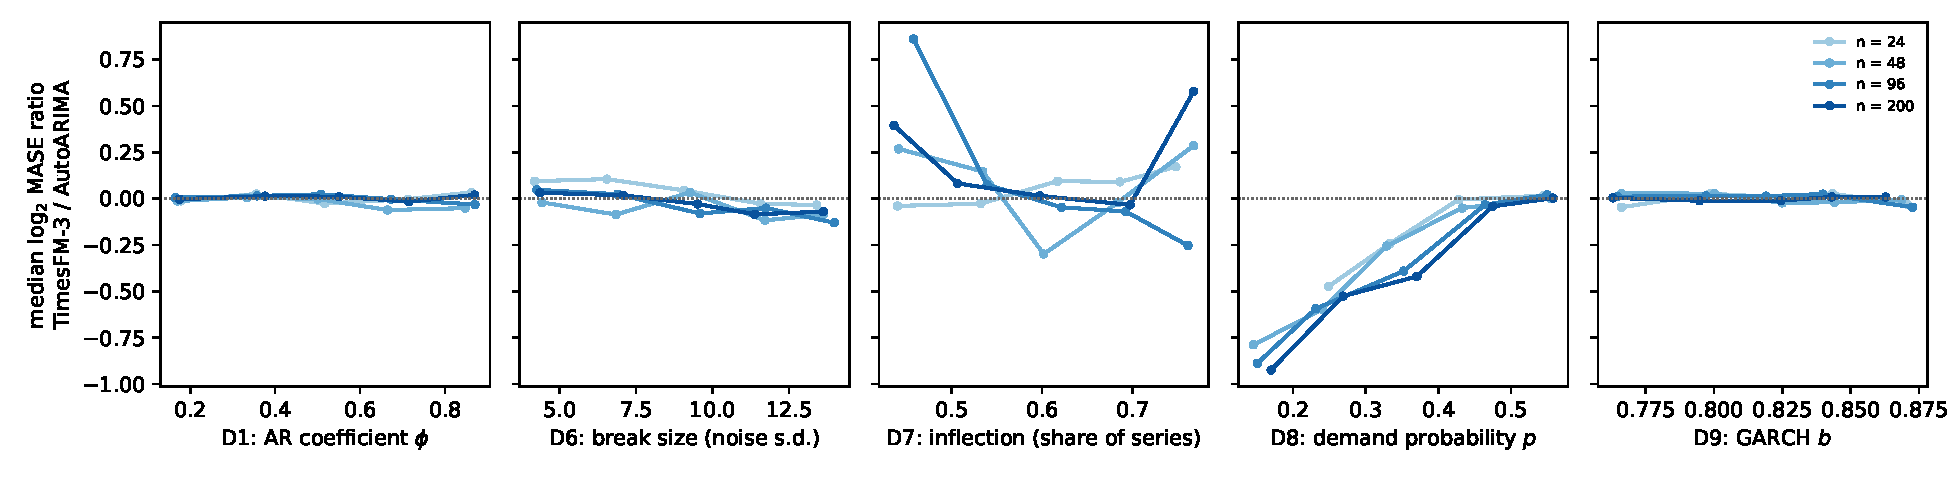
\includegraphics[width=\textwidth]{../figures/fig12_parameter_response.pdf}
\caption{Median $\log_2$ ratio of the MASE of TimesFM-3 to that of AutoARIMA, by quintile of the drawn
parameter, randomised-parameter design with Gaussian innovations. Values below zero favour TimesFM-3. For D8
the ratio compares median-type forecasts and is shown for completeness only.}
\label{fig:si-response}
\end{figure}

% generated by code/09_make_tables.py -- do not edit by hand
\begin{table}[!htbp]
\centering
\begin{threeparttable}
\caption{Mean MASE over $h = 1,\dots,12$ across 200 replications per cell.}
\label{tab:mase}
\small\setlength{\tabcolsep}{3pt}
\begin{tabular}{llrrrrrr}
\toprule
DGP & $n$ & Seas.\ naive & Theta & AutoETS & AutoARIMA & Combin. & \textbf{TimesFM-3} \\
\midrule
D1 (ARIMA) & 24 & 1.646 & 1.682 & 1.568 & 1.485 & 1.538 & \textbf{1.417} \\
 & 48 & 1.625 & 1.586 & 1.570 & 1.415 & 1.478 & \textbf{1.381} \\
 & 96 & 1.626 & 1.572 & 1.564 & 1.324 & 1.435 & \textbf{1.307} \\
 & 200 & 1.615 & 1.576 & 1.576 & 1.266 & 1.417 & \textbf{1.254} \\
\addlinespace
D2 (ARIMA) & 24 & 1.905 & 2.003 & 1.886 & 1.708 & 1.788 & \textbf{1.675} \\
 & 48 & 1.838 & 1.860 & 1.834 & 1.575 & 1.688 & \textbf{1.518} \\
 & 96 & 1.810 & 1.812 & 1.811 & 1.517 & 1.643 & \textbf{1.455} \\
 & 200 & 1.922 & 1.919 & 1.921 & \textbf{1.374} & 1.654 & 1.383 \\
\addlinespace
D3 (ARIMA) & 24 & \textbf{4.411} & 4.483 & 4.892 & 5.275 & 4.659 & 4.656 \\
 & 48 & 4.252 & \textbf{4.179} & 4.547 & 4.679 & 4.313 & 4.274 \\
 & 96 & 4.125 & 4.135 & 3.938 & 3.940 & \textbf{3.871} & 4.023 \\
 & 200 & 4.512 & 4.427 & 4.275 & \textbf{4.195} & 4.199 & 4.297 \\
\addlinespace
D4 (ARIMA) & 24 & \textbf{1.029} & 4.146 & 3.602 & 2.284 & 3.084 & 1.321 \\
 & 48 & 1.021 & 1.944 & 1.720 & \textbf{1.014} & 1.395 & 1.295 \\
 & 96 & 1.005 & 2.910 & 2.407 & \textbf{0.886} & 1.839 & 1.124 \\
 & 200 & 1.053 & 4.155 & 1.085 & \textbf{0.886} & 1.700 & 1.161 \\
\addlinespace
D5 (ETS) & 24 & \textbf{1.139} & 3.154 & 3.025 & 1.574 & 2.474 & 1.152 \\
 & 48 & 1.108 & 0.956 & 0.741 & \textbf{0.717} & 0.731 & 0.815 \\
 & 96 & 1.076 & 0.757 & 0.761 & 0.732 & \textbf{0.713} & 0.761 \\
 & 200 & 1.040 & 0.759 & 0.681 & \textbf{0.626} & 0.645 & 0.689 \\
\addlinespace
D6 (none) & 24 & 0.801 & 1.327 & \textbf{0.766} & 0.802 & 0.837 & 0.807 \\
 & 48 & 0.947 & 1.115 & 0.869 & 0.925 & 0.924 & \textbf{0.825} \\
 & 96 & 1.006 & 0.963 & 0.905 & 0.920 & 0.916 & \textbf{0.865} \\
 & 200 & 0.934 & 0.840 & \textbf{0.825} & 0.833 & 0.827 & 0.844 \\
\addlinespace
D7 (none) & 24 & 5.417 & 3.179 & 1.272 & \textbf{1.083} & 1.680 & 1.142 \\
 & 48 & 4.243 & 2.262 & 1.602 & 1.076 & 0.970 & \textbf{0.751} \\
 & 96 & 1.655 & \textbf{0.821} & 1.305 & 1.329 & 1.097 & 0.959 \\
 & 200 & \textbf{0.917} & 1.301 & 0.966 & 0.994 & 0.954 & 0.933 \\
\addlinespace
D8 (none) & 24 & 1.019 & 0.999 & 1.047 & 0.996 & 1.010 & \textbf{0.780} \\
 & 48 & 1.066 & 0.984 & 0.988 & 0.962 & 0.974 & \textbf{0.708} \\
 & 96 & 0.932 & 0.923 & 0.926 & 0.924 & 0.923 & \textbf{0.683} \\
 & 200 & 1.005 & 0.943 & 0.939 & 0.939 & 0.940 & \textbf{0.694} \\
\addlinespace
D9 (ARIMA (mean only)) & 24 & 1.547 & 1.518 & 1.454 & 1.372 & 1.404 & \textbf{1.321} \\
 & 48 & 1.588 & 1.486 & 1.476 & 1.244 & 1.353 & \textbf{1.239} \\
 & 96 & 1.430 & 1.342 & 1.333 & \textbf{1.098} & 1.213 & 1.104 \\
 & 200 & 1.577 & 1.503 & 1.504 & \textbf{1.190} & 1.341 & 1.200 \\
\bottomrule
\end{tabular}
\begin{tablenotes}[flushleft]\footnotesize
\item \textit{Note:} Lower is better; the best method in each row is in bold. The family in parentheses after each process label is the one correctly specified for it by construction.
\end{tablenotes}
\end{threeparttable}
\end{table}


\section{Supplementary diagnostics}
\label{si:diagnostics}

\tableref{tab:si-worst} summarises each method's ratio to the best method of a cell with and without the
two cells in which only two seasonal cycles are observed (D4 and D5 at $n = 24$). \tableref{tab:si-forms}
lists the model forms chosen by AutoETS and AutoARIMA on the seasonal processes at $n = 24$ and $n = 48$,
and \tableref{tab:si-is} gives the 80\% interval score by process. Pooling all 180 tests of the
$h = 1$--12 slice into one Benjamini--Hochberg family gives 134 significant comparisons, 115 won by
TimesFM-3 (13--9 against AutoARIMA); pooling all 540 tests gives 132 and 113 (12--9), against 132 and 113
(11--9) with the pre-registered families.

\begin{table}[!htbp]
\centering
\begin{threeparttable}
\caption{Ratio of each method's mean MASE to the best in the same cell, with and without the two-cycle cells.}
\label{tab:si-worst}
\small\setlength{\tabcolsep}{4pt}
\begin{tabular}{lcccccl}
\toprule
Method & Median & Geom.\ mean & 90th pct. & Worst & Worst excl. & Cell of worst excl. \\
\midrule
Seasonal naive & 1.200 & 1.331 & 1.60 & 5.65 & 5.65 & D7, $n = 48$ \\
Theta & 1.251 & 1.458 & 2.97 & 4.69 & 4.69 & D4, $n = 200$ \\
AutoETS & 1.194 & 1.296 & 1.91 & 3.50 & 2.72 & D4, $n = 96$ \\
AutoARIMA & 1.032 & 1.118 & 1.37 & 2.22 & 1.62 & D7, $n = 96$ \\
Combination & 1.108 & 1.228 & 1.74 & 3.00 & 2.08 & D4, $n = 96$ \\
TimesFM-3 & 1.008 & 1.050 & 1.22 & 1.31 & 1.31 & D4, $n = 200$ \\
\bottomrule
\end{tabular}
\begin{tablenotes}[flushleft]\footnotesize
\item \textit{Note:} Main design, 36 cells, $h = 1, \dots, 12$. ``Excl.'' leaves out D4 and D5 at $n = 24$, where only two seasonal cycles are observed; the 90th percentile is taken over the 36 cells.
\end{tablenotes}
\end{threeparttable}
\end{table}

\begin{table}[!htbp]
\centering
\begin{threeparttable}
\caption{Model forms chosen by AutoETS and AutoARIMA on the seasonal processes, given $m = 12$.}
\label{tab:si-forms}
\scriptsize\setlength{\tabcolsep}{4pt}
\begin{tabular}{llccp{4.3cm}p{4.3cm}}
\toprule
Process & $n$ & ETS seas.\ (\%) & ARIMA seas.\ (\%) & Most frequent ETS forms & Most frequent ARIMA orders \\
\midrule
D4 & 24 & 8.5 & 0.0 & ETS(A,N,N) (100), ETS(M,N,N) (83), ETS(A,N,A) (8) & (2,0,1)(0,0,0) (52), (3,0,1)(0,0,0) (44) \\
D4 & 48 & 98.0 & 100.0 & ETS(A,N,A) (67), ETS(M,N,M) (60), ETS(M,N,A) (42) & (1,0,0)(1,1,0) (52), (1,0,0)(0,1,1) (26) \\
D5 & 24 & 0.0 & 0.0 & ETS(A,N,N) (117), ETS(M,N,N) (83) & (2,0,1)(0,0,0) (72), (4,0,0)(0,0,0) (52) \\
D5 & 48 & 100.0 & 100.0 & ETS(M,N,M) (54), ETS(A,A,A) (40), ETS(M,A,A) (26) & (0,1,1)(0,1,1) (48), (0,0,0)(0,1,1) (35) \\
\bottomrule
\end{tabular}
\begin{tablenotes}[flushleft]\footnotesize
\item \textit{Note:} 200 replications per row, the series of the main design; counts out of 200 in parentheses. A form is seasonal when it has a seasonal component (ETS) or a non-zero seasonal order (ARIMA).
\end{tablenotes}
\end{threeparttable}
\end{table}

\begin{table}[!htbp]
\centering
\begin{threeparttable}
\caption{Scaled 80\% interval score by process, averaged over the four lengths.}
\label{tab:si-is}
\small\setlength{\tabcolsep}{4pt}
\begin{tabular}{lcccccc}
\toprule
Process & Seasonal naive & Theta & AutoETS & AutoARIMA & Combination & TimesFM-3 \\
\midrule
D1 & 8.49 & 7.80 & 7.67 & 6.36 & 6.97 & \textbf{6.05} \\
D2 & 9.05 & 9.28 & 9.09 & 6.98 & 8.00 & \textbf{6.86} \\
D3 & 23.33 & 23.31 & 22.12 & 22.03 & \textbf{21.01} & 21.24 \\
D4 & \textbf{4.58} & 16.77 & 11.04 & 5.65 & 9.65 & 5.69 \\
D5 & 4.64 & 7.22 & 6.51 & 4.29 & 5.59 & \textbf{3.98} \\
D6 & 9.35 & 7.13 & 7.21 & 7.53 & 7.28 & \textbf{4.55} \\
D7 & 14.14 & 8.59 & 5.91 & 5.17 & 5.51 & \textbf{4.55} \\
D8 & 10.11 & 4.60 & 4.50 & 4.40 & 4.47 & \textbf{3.54} \\
D9 & 8.56 & 7.22 & 7.07 & 5.82 & 6.44 & \textbf{5.67} \\
\bottomrule
\end{tabular}
\begin{tablenotes}[flushleft]\footnotesize
\item \textit{Note:} Interval score of $[q_{0.1}, q_{0.9}]$ with $\alpha = 0.2$ (width plus $2/\alpha$ times the distance by which the outcome falls outside the interval), averaged over the horizon and scaled by the MASE denominator, as for MSIS; lower is better, the best in bold. TimesFM-3 has the lowest score in 22 of the 36 (process, length) cells.
\end{tablenotes}
\end{threeparttable}
\end{table}

\begin{table}[!htbp]
\centering
\begin{threeparttable}
\caption{Classical methods in \pkg{forecast} (R) and \pkg{StatsForecast} (Python) on the seasonal processes: mean MASE over $h = 1, \dots, 12$.}
\label{tab:si-rcheck}
\footnotesize\setlength{\tabcolsep}{4pt}
\begin{tabular}{llccccccc}
\toprule
Process & $n$ & R ARIMA & SF ARIMA & R ETS & SF ETS & R Theta & SF Theta & R seas.\ (\%) \\
\midrule
D4 & 24 & 2.866 & 2.284 & 3.949 & 3.602 & 4.140 & 4.146 & 0 / 13 \\
D4 & 48 & 1.008 & 1.014 & 1.765 & 1.720 & 1.949 & 1.944 & 100 / 100 \\
D4 & 96 & 0.891 & 0.886 & 1.044 & 2.407 & 2.896 & 2.910 & 100 / 100 \\
D4 & 200 & 0.894 & 0.886 & 1.056 & 1.085 & 4.085 & 4.155 & 100 / 100 \\
D5 & 24 & 1.695 & 1.574 & 3.304 & 3.025 & 3.147 & 3.154 & 0 / 0 \\
D5 & 48 & 0.717 & 0.717 & 0.739 & 0.741 & 0.947 & 0.956 & 100 / 100 \\
D5 & 96 & 0.747 & 0.732 & 0.719 & 0.761 & 0.759 & 0.757 & 100 / 100 \\
D5 & 200 & 0.631 & 0.626 & 0.644 & 0.681 & 0.760 & 0.759 & 100 / 100 \\
\bottomrule
\end{tabular}
\begin{tablenotes}[flushleft]\footnotesize
\item \textit{Note:} The same 200 series per row. R: \code{auto.arima}, \code{ets} and \code{thetaf} of \pkg{forecast} 9.0.2 at their defaults, with frequency 12; SF: \pkg{StatsForecast} 2.1.1 as in the main text. R seas.: share of series given a seasonal form by \code{auto.arima} / \code{ets}. No R fit failed. On D4 at $n = 96$ \pkg{StatsForecast}'s AutoETS settles on a near-zero seasonal smoothing parameter with a much lower likelihood than R's fit of the same form.
\end{tablenotes}
\end{threeparttable}
\end{table}


\section{A longer horizon}
\label{si:h48}

The main design forecasts 12 steps. To see whether its conclusions depend on that choice, the nine
processes were regenerated with the same seeds at length $n + 48$ and forecast 48 steps ahead by the six
pre-registered methods, TimesFM-2.5 and Chronos-2 (post hoc). Because the inflection of D7 sits at
$0.6(n + H)$, the longer horizon moves it into the context for $n = 200$: the series has reached its plateau
before the forecast origin. \tableref{tab:si-h48} and Figure~S3 summarise the results.

\begin{table}[!htbp]
\centering
\begin{threeparttable}
\caption{Longer horizon ($H = 48$): worst ratio to the cell-best and 80\% coverage by block of steps.}
\label{tab:si-h48}
\small\setlength{\tabcolsep}{4pt}
\begin{tabular}{lccccccc}
\toprule
Method & \multicolumn{3}{c}{Worst ratio, D7 excluded} & \multicolumn{3}{c}{Coverage 80\%} & D7, $n = 200$ \\
 & 1--12 & 13--24 & 25--48 & 1--12 & 13--24 & 25--48 & MASE 1--48 \\
\midrule
TimesFM-3 & 1.31 & 1.39 & 1.80 & 0.788 & 0.774 & 0.760 & 8.37 \\
TimesFM-2.5 & 1.42 & 1.59 & 1.77 & 0.781 & 0.734 & 0.707 & 12.22 \\
Chronos-2 & 2.94 & 2.71 & 3.33 & 0.787 & 0.762 & 0.761 & 5.30 \\
AutoARIMA & 2.11 & 1.60 & 1.41 & 0.760 & 0.739 & 0.720 & 2.51 \\
AutoETS & 3.49 & 2.17 & 1.67 & 0.779 & 0.790 & 0.784 & 2.35 \\
Theta & 4.65 & 3.66 & 6.27 & 0.731 & 0.757 & 0.768 & 2.73 \\
Combination & 2.92 & 2.00 & 2.17 & 0.788 & 0.812 & 0.814 & 2.22 \\
Seasonal naive & 1.66 & 1.88 & 1.87 & 0.805 & 0.780 & 0.753 & 1.11 \\
\bottomrule
\end{tabular}
\begin{tablenotes}[flushleft]\footnotesize
\item \textit{Note:} The nine processes regenerated with the same seeds at length $n + 48$, 200 replications per cell; ratios to the best of the eight methods in each of the 32 (process, length) cells without D7. Coverage is averaged over all 36 cells. The last column is the mean MASE over the 48 steps on D7 at $n = 200$, where the process has reached its plateau before the forecast origin.
\end{tablenotes}
\end{threeparttable}
\end{table}


\begin{figure}[!htbp]
\centering
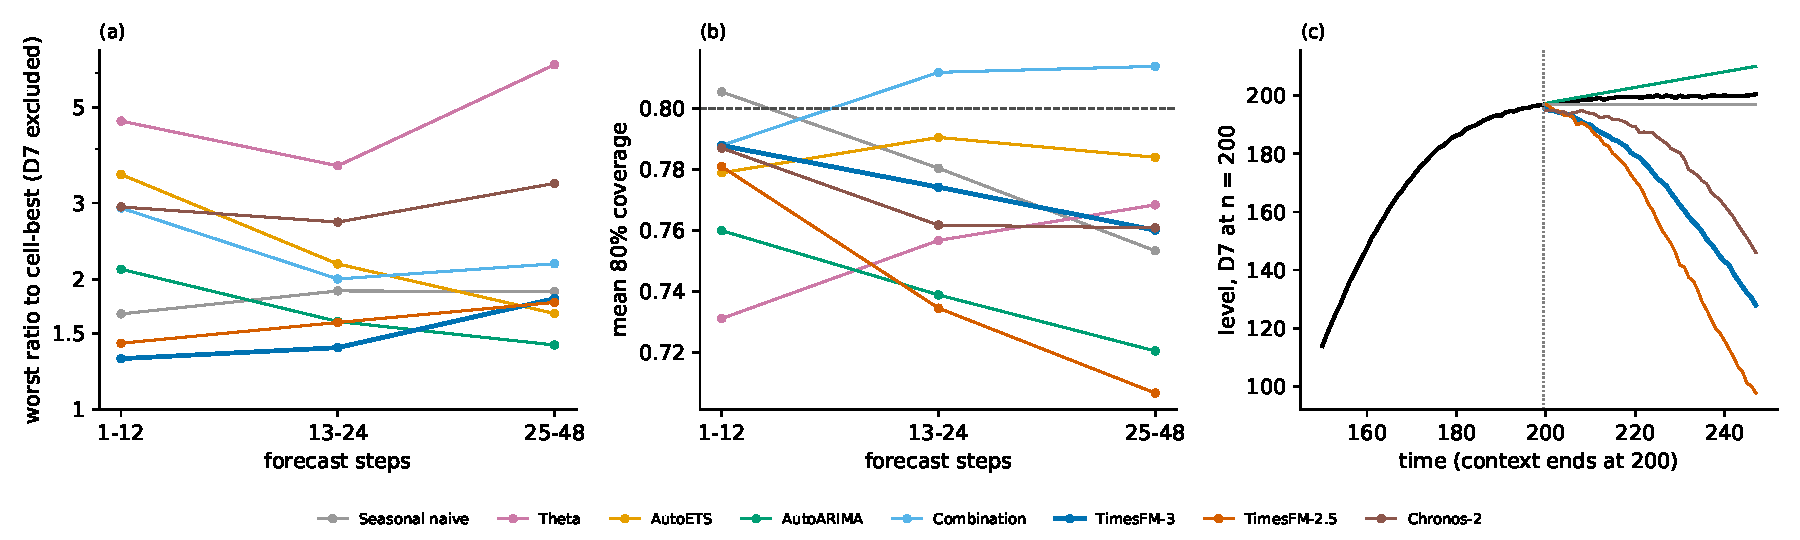
\includegraphics[width=\textwidth]{../figures/fig_si_h48.pdf}
\caption{Longer horizon ($H = 48$). (a) Worst ratio to the cell-best method by block of forecast steps, D7
excluded. (b) Mean coverage of the nominal 80\% intervals by block; the dashed line is the nominal level.
(c) D7 at $n = 200$: mean of the 200 series (black) and mean point forecasts over the 48 steps.}
\label{fig:si-h48}
\end{figure}

\end{document}
